\documentclass[a4paper,11pt,twoside]{book}

\usepackage[english]{babel}
\usepackage{setspace}
\usepackage[utf8]{inputenc}
\usepackage{graphicx}
\usepackage{pdfpages}
\usepackage{longtable}
\usepackage{url}
\urlstyle{tt}

\usepackage[T1]{fontenc}
\usepackage[utf8]{inputenc}
\usepackage{hyperref}
\usepackage{fullpage}
\usepackage{fancyhdr}


\hypersetup{
     colorlinks = true, linkcolor = blue,
     citecolor   = blue,
     urlcolor    = blue,
}


\usepackage{tocloft}
\renewcommand{\cftpartleader}{\cftdotfill{\cftdotsep}} % for parts
\renewcommand{\cftchapleader}{\cftdotfill{\cftdotsep}} % for chapters
\renewcommand{\cftsecleader}{\cftdotfill{\cftdotsep}} % for sections

\renewcommand{\headrulewidth}{0pt}

\newcommand{\newoddpage} {\clearpage
  \ifthenelse{\isodd{\value{page}}}{}
  {\thispagestyle{empty}\quad\newpage}}

\newcommand{\addpaper}[5]{% #1 path; #2 label; #3 authors; #4 title; #5 URL
  \newoddpage
  \phantomsection
  \addcontentsline{toc}{section}{#3. \emph{#4}}  

\thispagestyle{fancy} %
  
  % scriptsize / tiny
  %\lfoot{\scriptsize {\tiny Martins, Moniz, Fumega, Martins, Batista, Coheur, Parra, Trancoso, Turchi, Bisazza, Moorkens, Guerberof, Nurminen, Marg, Forcada (eds.)}\\
  \lfoot{\scriptsize {\tiny Macken, Rufener, Van den Bogaert, Daems, Tezcan, Vanroy, Fonteyne, Barrault, Costa-jussà, Kemp, Pilos, Declercq, Koponen, Forcada, Scarton, Moniz (eds.)}\\
    {\em Proceedings of the 23rd Annual Conference of the European Association for Machine Translation}, p. \pageref{beg#2}--\pageref{end#2}\\
      Ghent, Belgium, June 2022. %\url{#5}
  }
  \cfoot{}
  %
  \label{beg#2}
  \includepdf[pages={1},pagecommand={},fitpaper=true,trim=0 0 0 0,
  offset=0 0, turn=true,noautoscale=true]{#1}
  %
  \pagestyle{fancy} %
  \lfoot{} %
  \cfoot{\thepage} 
  %
  \includepdf[pages={2-},pagecommand={\label{end#2}},fitpaper=true,trim=0 0
  0 0, offset=0 0,turn=true,noautoscale=true]{#1}
}


\newcommand{\addproject}[5]{% #1 path; #2 label; #3 authors; #4 title;
                          % #5 URL
  \newoddpage
  \phantomsection
  \addcontentsline{toc}{section}{#3. \emph{#4}}  
  \thispagestyle{fancy} %
  \lfoot{\scriptsize {\tiny Macken, Rufener, Van den Bogaert, Daems, Tezcan, Vanroy, Fonteyne, Barrault, Costa-jussà, Kemp, Pilos, Declercq, Koponen, Forcada, Moniz (eds.)}\\
    {\em Proceedings of the 23rd Annual Conference of the European Association for Machine Translation}, p. \pageref{beg#2}\\
      Ghent, Belgium, June 2022. %\url{#5}
  }
  \cfoot{}
  %
  \label{beg#2}
  \includepdf[pages={1},pagecommand={},fitpaper=true,trim=0 0 0 0,
  offset=0 0, turn=true,noautoscale=true]{#1}
  %
  \pagestyle{fancy} %
  \lfoot{} %
  \cfoot{\thepage} 
}


\usepackage{calc}
\setlength{\footskip}{\paperheight
  -(1in+\voffset+\topmargin+\headheight+\headsep+\textheight)
  -0.6in}

\newcommand{\mychapter}[1]{
    \newpage
    \phantomsection{}
    \cfoot{}
    \vspace*{\fill}
    \begin{center}
    \begin{Huge}
    \textbf{#1}
    \end{Huge}
    \end{center}
    \addcontentsline{toc}{chapter}{#1}
    \vspace*{\fill}
    \newpage
    \cfoot{\thepage}
}

%%%%%%%%%%%%%%%%%%%%%%%%%%%%%%%%%%%%%%%%%%%%%%%%%%%%%%%%%%%%%%%828%%%%%%%%%%%%%%%%%

%\usepackage{draftwatermark}
%\SetWatermarkText{Draft}
%\SetWatermarkScale{1}

\begin{document}

\pagestyle{fancy} 
\lhead{}
\rhead{}
\chead{}
\lfoot{} 
\rfoot{} 
\cfoot{\thepage}

\newoddpage
\thispagestyle{empty}
\enlargethispage{1cm}
\begin{center}
\phantom{x}
\vspace{-2cm}

\includegraphics[width=0.8\columnwidth]{logos/eamt2022-gent.png}

\vspace{1cm}

{\huge Proceedings of the}\\[2ex]
\textbf{\huge 23rd Annual Conference of \\[0.2ex]
  the European Association\\[1.0ex] for Machine Translation} 
  
\vspace{1.5cm}

{\LARGE 1 -- 3 June 2022\\[0.75ex]Ghent, Belgium}
\vspace{3cm}

\textbf{\em Edited by}

\vspace{1em}
Lieve Macken,
Andrew Rufener,
Joachim Van den Bogaert,
Joke Daems,
Arda Tezcan,
Bram Vanroy,
Margot Fonteyne,
Loïc Barrault,
Marta R. Costa-jussà,
Ellie Kemp,
Spyridon Pilos,
Christophe Declercq,
Maarit Koponen,
Mikel L. Forcada,
Carolina Scarton,
Helena Moniz

%\vspace{1cm}
\vfill

\textbf{\em Organised by}

\vspace{1em}
\begin{tabular}{ccc}
\begin{tabular}{l}
\includegraphics[width=0.28\columnwidth]{logos/lt3-text-logo.png}
\end{tabular} 
&
\begin{tabular}{c}
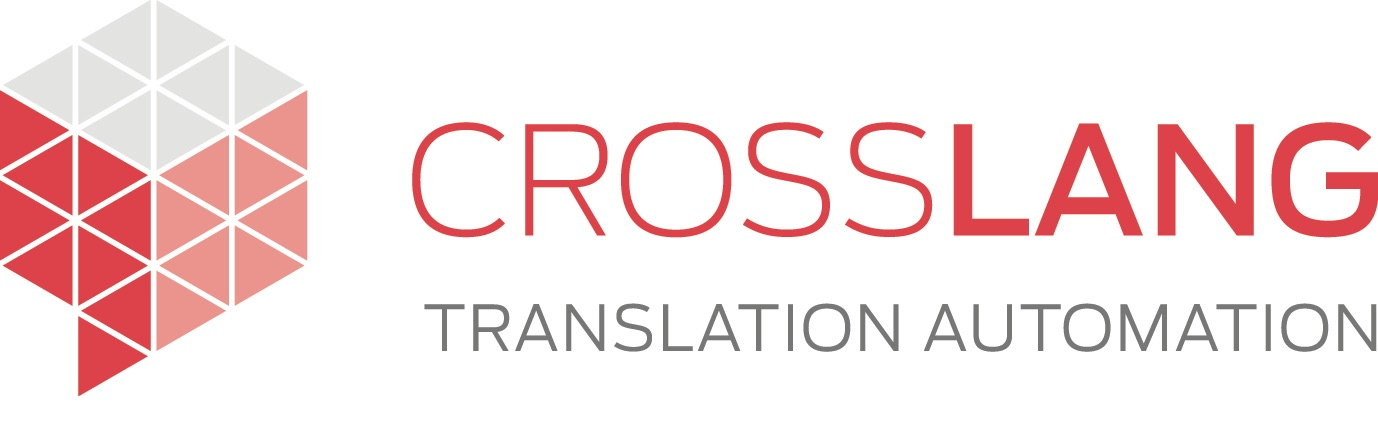
\includegraphics[width=0.35\columnwidth]{logos/crosslang-logo.png}
\end{tabular} 
&
\begin{tabular}{r}
\includegraphics[width=0.18\columnwidth]{logos/ugent-logo.png}\\
\end{tabular} 
\end{tabular}
\end{center}

\newoddpage
\thispagestyle{empty}
\vfill \mbox{} \vfill

\begin{onehalfspacing}

\noindent 
\includegraphics[scale=0.5]{logos/creative_commons.pdf} 
\vspace{1em}

\noindent 
The papers published in this proceedings are ---unless indicated
otherwise--- covered by the Creative Commons
Attribution-NonCommercial-NoDerivatives 3.0 International (CC-BY-ND
3.0). You may copy, distribute, and transmit the work, provided that
you attribute it (authorship, proceedings, publisher) in the manner
specified by the author(s) or licensor(s), and that you do not use it
for commercial purposes. The full text of the licence may be found at
\url{https://creativecommons.org/licenses/by-nc-nd/3.0/deed.en}.

\vspace{1cm}

\noindent © 2022 The authors\\
\noindent \textbf{ISBN:} 9789464597622\\

\end{onehalfspacing}

\vfill \mbox{}

%%%%%%%%%%%%%%%%%%%%%%%%%%%%%%%%%%%%%%%%%%%%%%%%%%%%%%%%%%%%%%%%%%%%%%%%%%%%%%%%

\newoddpage
\frontmatter

\tableofcontents


\chapter*{Foreword from the General Chair}
\addcontentsline{toc}{chapter}{Foreword from the General Chair}
%\vspace{-0.8cm}

\begin{onehalfspacing}
As president of the European Association for Machine Translation (EAMT) and General Chair of the 23rd Annual Conference of the EAMT, it is with great pleasure that I write these opening words to the Proceedings of EAMT 2022 (a first time for me!). The preparations for EAMT 2022 were initially started by the former President, Mikel Forcada, to whom I am deeply grateful for all the assistance and hand over.

A first note of appreciation and gratitude to the Executive Board Members who have moved to new plans in life, after long and outstanding dedicated service to the EAMT community. Firstly, Tony Clarke, EAMT treasurer for 23 years, in appreciation for his invaluable service as the longest-standing treasurer of our Association. To Andy Way, in appreciation for his years of service as secretary, president, conference organizer, and member of the Executive Board of our Association. To Viggo Hansen, our gratitude for his years of service as secretary, conference organizer, and member of the Executive Board of our Association. 

One of the most significant milestones this year was the John Hutchins Machine Translation Archive new domain, an achievement built upon the hard work of our former president, Mikel Forcada, and a group of dedicated members, Barry Haddow, Leopoldo Pla, and Matt Post. The John Hutchins Machine Translation Archive is alive at: \url{https://mt-archive.net/}. We invite our community to visit John's archive!

A few lines more of gratitude to Matt Post, for being responsible for the import of the MT Archive conference proceedings into the ACL anthology. Our community is very thankful to Matt Post for the massive import work and patience along the way!

Now our EAMT 2022 event! After an online-edition in Lisbon, in 2020 (in which I had no opportunity to welcome you in person as a co-chair) and a cancellation in 2021, we now move forward to a fully and much hoped for live event in Ghent, Belgium! Winds of change in the pandemics are bringing a new hope. Embedded in this spirit, the local organizers are enthusiastic about hosting an in-person event, after the two-years interregnum, anticipating a much needed gathering of the community. Let us hope that these changes are here to stay. 

Despite the positive changes in terms of covid, our community reached out to us requesting for support, specifically for freelance translators and/or members from low-income areas and war zones. For the first time, we have opened two calls for grants, encompassing, on one hand, students from Translation Studies and, on another, members from Middle East and African countries. A total of seven grants were given. We hope this initiative may mitigate the hard times we are living and may bring richer discussions into our EAMT 2022, diversifying geographically our membership.

EAMT 2022 will have a three-day, four-track programme put together by our chairs: Löic Barrault and Marta Costa-Jussà, research track co-chairs; Ellie Kemp and Spyridon Pilos, user track co-chairs; Maarit Koponen and Christophe Declercq, translator track co-chairs; and Mikel Forcada, as the projects/products track chair. Carolina Scarton, Secretary of EAMT, was the chair of the Best Thesis Award and also the technical coordinator of the reviewing process (our gratitude to Carolina who is always willing to support our community).

This year, the programme will also include two keynotes speakers, invited by Lieve Macken and Andrew Rufener (with our full support and enthusiasm), Laura Rossi (Medtronic) and Jörg Tiedemann (University of Helsinki), combining industry and academia visions on the field, a true honour to have them and to be able to discuss their talks in person.

EAMT 2022 brings a new breeze of hope and it is the result of the hard work of our local organizers from the Language and Translation Technology Team (LT3) of Ghent University and CrossLang. Our gratitude and appreciation to the LT3 team, Lieve Macken (co-chair), Joke Daems, Arda Tezcan, and Bram Vanroy; and to the CrossLang team, Andrew Rufener (co-chair), Joachim Van den Bogaert, and especially to Martine Massiera for her outstanding work taking care of our sponsors, registration process, all social events, and smoothly handling the logistics of the new calls for grants. 

EAMT has been supported by generous sponsors in its initiatives along the years. This year is no exception. Our gratitude to our sponsors: Microsoft (platinum sponsor, who will also be giving a talk entitled ``Microsoft and Translators' quest to break down language barriers''), Pangeanic and Yamagata (silver sponsors), STAR Group and Unbabel (bronze sponsors), Apertium (collaborator sponsor), Springer (best paper award supporter) and MultiLingual (media sponsor).

A final note to our participants! By the time I am writing these lines, there are already 113 participants and the number continues growing! Even in unstable times, this number is a very positive sign! We can finally meet in person! Let us take this opportunity to revive fruitful discussions, scientific collaborations, and constructive feedback in our community. I'm looking forward to seeing you all, finally!


\end{onehalfspacing}

\vspace{1cm}

\noindent Lisboa, 2022

\vspace{0.5cm}

\noindent \textbf{Helena Moniz}

\noindent President of the EAMT

\noindent General Chair of EAMT 2022

\noindent University of Lisbon / INESC-ID, Portugal



\chapter*{Message from the Organising Committee Chairs}
\addcontentsline{toc}{chapter}{Message from the Organising Committee Chairs}
%\vspace{-0.9cm}


\begin{onehalfspacing}
It is with great pleasure that we finally welcome you in Ghent to attend the 23rd Annual Conference of the European Association for Machine Translation.
 
The idea of organizing the 23rd Annual Conference of EAMT in Ghent jointly by the LT3 research team and CrossLang emerged in 2019 at the Croke Park stadium in Dublin where we enjoyed the Gala Dinner of the MT Summit. Unfortunately, COVID-19 prevented us from organizing an on-site event and EAMT2021 was first postponed and eventually cancelled. We are therefore extremely pleased to be able to welcome you all in our beautiful city for EAMT2022 and to meet you all in person.
 
A lot can happen in two years. The venue we had originally booked, the Aula Academica of Ghent University, a historic building of 1826, was no longer available due to renovation work. As Ghent is a great mix of old and new, we instead welcome you in the trendy Zebrastraat and keep the historic part for the conference dinner, which will be organized in the church of Monasterium PoortAckere. 
 
People also change jobs. With a new team (and a new EAMT president) we continued the preparations for the conference. We kept the basic format of previous editions, but added a second keynote speaker. This not only allowed us to find the optimal balance between academia and industry but also ensured gender balance. We are really looking forward to the talks of Jörg Tiedemann and Laura Rossi.
 
We did not opt for a hybrid conference as the advantages did not outweigh the disadvantages. As a compromise, we will record the oral sessions and make the recordings available after the conference. 
 
We would express our sincerest gratitude to everyone who made EAMT2022 possible: Mikel Forcada as former president of EAMT; Helena Moniz as new president of EAMT; Carolina Scarton as EAMT Secretary; Löic Barrault and Marta Costa-Jussà as research track chairs; Ellie Kemp and Spyridon Pilos as user track co-chairs; Maarit Koponen and Christophe Declercq as translator track chairs.  
 
We extend our thanks to our sponsors for their invaluable support: Microsoft (Platinum sponsor), Pangeanic and Yamagata (Silver sponsors), STAR Group and Unbabel (Bronze sponsors), Apertium (Collaborator sponsor), Springer (Supporter sponsor), and MultiLingual (media sponsor).
 
This conference would not have been possible without the hard work of all members of the joint organizing team: Andrew Rufener, Martine Massiera and Joachim Van den Bogaert of CrossLang; Lieve Macken, Joke Daems, Arda Tezcan, Bram Vanroy and Margot Fonteyne of the Language and Translation Technology Team (LT³) of Ghent University. Sincere thanks as well to Sam Delmotte of Ghent University for recording the oral sessions.

\end{onehalfspacing}

\vspace{1cm}
\begin{center}
\begin{tabular}{p{5cm}p{5cm}}
\textbf{Lieve Macken} & \textbf{Andrew Rufener}\\
Ghent University, LT³ & CrossLang\\
\end{tabular}
\vspace{0.5cm}
\\
\noindent On behalf of the local organizers
\end{center}


\chapter*{Preface by the Programme Chairs}
\addcontentsline{toc}{chapter}{Preface by the Programme Chairs}


\begin{onehalfspacing}
On behalf of the programme chairs, a warm welcome to the 23rd annual conference of the European Association for Machine Translation in Ghent, Belgium. After all the restrictions, rescheduling and cancellations of events in the past couple of years, and after a prolonged period with almost all meetings online, we are delighted to finally be meeting our colleagues face-to-face again!

Following the approach which has proven so successful in the previous editions of EAMT, the conference programme consists of papers and posters divided into four tracks. These relate to research, users, translators and projects/products.

The research track this year was one of the most competitive tracks ever in the history of EAMT. Only 17 out of 39 papers were accepted (an acceptance rate of 44\%), based on three-peer reviews. The papers describe state-of-the-art work being conducted and, therefore, are highly relevant to our community.  Eight papers will be presented orally and nine as posters, as you may already find in the programme. We invite our community to reach out to the authors and discuss the relevant work conducted in such a demanding track.

The submissions for the user track in this edition mostly tackle the customer support domain - a particular focus of the oral sessions of the programme - and industry usage of MT. This track will discuss a number of practical issues for users. These range from the notion of “users” in a very challenging domain, to conversational data with strict time constraints, and the quality of the MT produced.

The translator's track, as is evident from the name, emphasises the perspective of translators on MT. This year, the track features three peer-reviewed papers, each of which addresses aspects of machine translation and post-editing carried out by translators in different settings. The diverging uses of post-editing and machine translation cover a survey of corporate use of post-editing and revision in the NMT era, post-editing practices for automatically generated subtitles, and annotation of post-editing and machine translation errors using speech-to-text technology.

Forty-four papers were submitted to the largest ever project/product track in the history of EAMT conferences. Of them, 41 were eventually accepted, some of them after an additional round of improvements with the general audience of EAMT in sight. As these lines are written, authors are preparing their posters, and also their poster booster slides, in anticipation of their (strictly-timed) two minutes of glory before the poster session.

In addition to the papers and posters relating to the different tracks, the programme also features two fascinating invited talks: Laura Rossi with her talk titled ``I once said to my boss `SMT will never work...' '' and Jörg Tiedemann with ``Democratizing machine translation with OPUS-MT''.

We wish to thank the members of the scientific programme committee for their time and support, and for their invaluable expertise in peer-reviewing the submissions. Our thanks naturally go to all the authors, without whom the programme would not exist, the local organisers for all their hard work, as well as Carol Scarton, Helena Moniz and Mikel Forcada for their unfailing advice and support. 
\end{onehalfspacing}

\vspace{1cm}
\begin{center}
\begin{tabular}{p{7.5cm}p{7.5cm}}
\textbf{Löic Barrault} & \textbf{Marta Costa-jussà}\\
META AI Research & META AI Research\\\\
\textbf{Ellie Kemp} & \textbf{Spyridon Pilos}\\
CLEAR Global	 & European Court of Auditors\\\\
\textbf{Christophe Declercq} & \textbf{Maarit Koponen}\\
Univ. of Utrecht \&
Univ. College London	 & University of Eastern Finland\\\\
\textbf{Mikel Forcada} & \\
Universitat d'Alacant	 & 
\end{tabular}
\end{center}


\chapter*{EAMT 2022 Committees}
\addcontentsline{toc}{chapter}{EAMT 2022 Committees}

\section*{General Chair}
\noindent Helena Moniz, University of Lisbon, INESC-ID


\section*{Programme Chairs}
\subsection*{Research track}
\noindent Loïc Barrault, META AI Research\\
\noindent Marta R. Costa-jussà, META AI Research

\subsection*{User track}
\noindent Ellie Kemp, CLEAR Global\\
\noindent Spyridon Pilos, European Court of Auditors

\subsection*{Translators' track}
\noindent Christophe Declercq, Univ. of Utrecht \&
Univ. College London\\
\noindent Maarit Koponen, Univ. of Eastern Finland

\subsection*{Project/Product track}
\noindent Mikel L. Forcada, Univ. d'Alacant

\subsection*{Thesis award}
\noindent Carolina Scarton, Univ. of Sheffield

\section*{Organising committee}
\noindent Lieve Macken, LT3, Ghent University (co-chair)\\
\noindent Andrew Rufener, CrossLang (co-chair)\\
\noindent Joachim Van den Bogaert, CrossLang\\
\noindent Joke Daems, LT3, Ghent University\\
\noindent Arda Tezcan, LT3, Ghent University\\
\noindent Bram Vanroy, LT3, Ghent University\\
\noindent Margot Fonteyne, LT3, Ghent University\\



\pagebreak

\section*{Programme Committee}
\subsection*{Research track}

\noindent Duygu Ataman, New York University\\
\noindent Parnia Bahar, RWTH Aachen University\\
\noindent Anabela Barreiro, INESC-ID\\
\noindent Luisa Bentivogli, Fondazione Bruno Kessler\\
\noindent Magdalena Biesialska, Universitat Politècnica de Catalunya\\
\noindent José G. C. de Souza, Unbabel\\
\noindent Michael Carl, Kent State University\\
\noindent Sheila Castilho, Dublin City University\\
\noindent Mauro Cettolo, FBK - Fondazione Bruno Kessler\\
\noindent Colin Cherry, Google Research\\
\noindent Vishal Chowdhary, Microsoft\\
\noindent Chenhui Chu, Kyoto University\\
\noindent Raj Dabre, IIT Bombay\\
\noindent Mattia Antonino Di Gangi, AppTek\\
\noindent Miguel Domingo, Universitat Politècnica de València\\
\noindent Miquel Espla-Gomis, Universitat d'Alacant\\
\noindent Catarina Farinha, Unbabel\\
\noindent Mireia Farrús, Universitat de Barcelona\\
\noindent George Foster, Google\\
\noindent Mercedes García-Martínez, Pangeanic SL\\
\noindent Jesús González-Rubio, WebInterpret\\
\noindent Barry Haddow, The University of Edinburgh\\
\noindent Felix Hieber, Amazon\\
\noindent Matthias Huck, SAP SE\\
\noindent Shankar Kumar, Google\\
\noindent Ekaterina Lapshinova-Koltunski, Saarland University\\
\noindent Samuel Läubli, Zurich University of Applied Sciences\\
\noindent Lieve Macken, Ghent University\\
\noindent Andreas Maletti, Universität Leipzig\\
\noindent Joss Moorkens, Dublin City University\\
\noindent Mathias Müller, University of Zurich\\
\noindent Masaaki Nagata, NTT\\
\noindent Toshiaki Nakazawa, The University of Tokyo\\
\noindent Jan Niehues, Maastricht University\\
\noindent André Niyongabo, Polytechnic University of Catalonia\\
\noindent Constantin Orasan, University of Surrey\\
\noindent Pavel Pecina, Charles University\\
\noindent Stephan Peitz, Apple\\
\noindent Sergio Penkale, Unbabel\\
\noindent Andrei Popescu-Belis, HEIG-VD / HES-SO\\
\noindent Maja Popovic, ADAPT Centre @ DCU\\
\noindent Celia Rico, Universidad Complutense de Madrid, Spain\\
\noindent Matīss Rikters, Tilde\\
\noindent Rudolf Rosa, Charles University\\
\noindent Felipe Sánchez-Martínez, Universitat d'Alacant\\
\noindent Germán Sanchis-Trilles, Sciling S.L.\\
\noindent Yves Scherrer, University of Helsinki\\
\noindent Rico Sennrich, University of Zurich\\
\noindent Patrick Simianer, Lilt, Inc.\\
\noindent Katsuhito Sudoh, Nara Institute of Science and Technology\\
\noindent Aleš Tamchyna, Memsource a. s.\\
\noindent Jörg Tiedemann, University of Helsinki\\
\noindent Antonio Toral, University of Groningen\\
\noindent Marco Turchi, Fondazione Bruno Kessler\\
\noindent Vincent Vandeghinste, Instituut voor de Nederlandse Taal, Leiden \& Centre for Computational Linguistics, KU Leuven\\
\noindent Sebastian Vincent, The University of Sheffield\\
\noindent Marion Weller-Di Marco, CIS - University of Munich\\
\noindent Deyi Xiong, Tianjin University\\
\noindent François Yvon, CNRS\\
\noindent Jiajun Zhang, Institute of Automation Chinese Academy of Sciences\\

\pagebreak

\subsection*{User track}

\noindent Nora Aranberri, University of the Basque Country\\
\noindent Adam Bittlingmayer, ModelFront\\
\noindent Vera Cabarrão, Unbabel\\
\noindent Federico Gaspari, Università per Stranieri ``Dante Alighieri'' di Reggio Calabria, Italy\\
\noindent Georg Kirchner, Dell Technologies\\
\noindent László János Laki, Hungarian Research Centre for Linguistics\\
\noindent Lena Marg, Welocalize\\
\noindent Mary Nurminen, Tampere University\\
\noindent Morgan O'Brien, Momentive AI\\
\noindent Niko Papula, Multilizer\\
\noindent Daniel Prou, European Commission\\
\noindent Steve Richardson, Brigham Young University\\
\noindent Laura Rossi, Medtronic\\
\noindent Marina Sánchez-Torrón, Unbabel\\
\noindent Yury Sharshov, TBSJ\\
\noindent Dimitar Shterionov, Tilburg University\\
\noindent Masaru Yamada, Rikkyo University\\

% \subsubsection*{Subreviewers}


\clearpage

\subsection*{Translators' track}
\noindent Khetam Al Sharou, Imperial College London\\
\noindent Dorothée Behr, GESIS - Leibniz Institute for the Social Sciences\\
\noindent Patrick Cadwell, Dublin City University\\
\noindent Ruben de La Fuente, PayPal\\
\noindent Gökhan Dogru, Universitat Autonoma de Barcelona\\
\noindent Maria Fernandez-Parra, Swansea University\\
\noindent Dorothy Kenny, Dublin City University\\
\noindent Caroline Lehr, Zurich University of Applied Sciences\\
\noindent Rudy Loock, Université de Lille, France, \& CNRS ``Savoirs, Textes, Langage'' research unit\\
\noindent Antoni Oliver, Universitat Oberta de Catalunya\\
\noindent David Orrego-Carmona, Aston University\\
\noindent Alessandra Rossetti, Universiteit Antwerpen\\
\noindent Caroline Rossi, Université Grenoble Alpes\\
\noindent María Del Mar Sánchez Ramos, Universidad de Alcala\\
\noindent Vilelmini Sosoni, Ionian University\\

\clearpage

\subsection*{Thesis award}

\noindent José G. C. de Souza, Unbabel\\
\noindent Vera Cabarrao, Unbabel Lda.; INESC-ID\\
\noindent Sheila Castilho, Dublin City University\\
\noindent Mirella De Sisto, Tilburg University\\
\noindent Mattia Antonino Di Gangi, AppTek\\
\noindent Miquel Esplà-Gomis, Universitat d'Alacant\\
\noindent Federico Gaspari, Dublin City University\\
\noindent Barry Haddow, University of Edinburgh\\
\noindent Ekaterina Lapshinova-Koltunski, Saarland University\\
\noindent Lieve Macken, Ghent University\\
\noindent Andre Martins, Unbabel\\
\noindent Maja Popovic, ADAPT Centre @ DCU\\
\noindent Celia Rico, Universidad Complutense de Madrid\\
\noindent Víctor M. Sánchez-Cartagena, Universitat d'Alacant\\
\noindent Marina Sánchez-Torrón, Unbabel\\
\noindent Arda Tezcan, Ghent University\\
\noindent Marco Turchi, Fondazione Bruno Kessler\\

\newoddpage
\mainmatter

\chapter*{Invited Speeches}
\addcontentsline{toc}{chapter}{Invited Speeches}
\label{invited}

\section*{Democratizing machine translation with OPUS-MT}
\textbf{Jörg Tiedemann}, University of Helsinki, Finland
\vspace{0.5cm}

The demand for translation is ever growing and this trend will not stop. Being able to access the same kind of information is a fundamental prerequisite for equality in society and translation plays a crucial role when fighting discrimination based on language barriers. Efficient tools and a better coverage of the linguistic diversity in the World are necessary to cope with the amount of material that needs to be handled. Our mission is to support the development of high quality tools for automatic and computer-assisted translation by providing open services and resources that are independent of commercial interests and profit-driven companies. Equal information access is a human right and not only a privilege for people who can pay for it. In this talk I will discuss the current state of OPUS-MT, our project on open neural machine translation and the challenges that we try to tackle with multilingual NLP, transfer learning and data augmentation. I will report about on-going work on knowledge distillation, the creation of compact models for real-time translation and our work on modularization of neural MT.


\section*{``I once said to my boss `SMT will never work...' ''}
\textbf{Laura Rossi}, Medtronic 
\vspace{0.5cm}

I once said to my boss: `SMT will never work...', yet here we are: after being statistical, MT became neural and even adaptive, and achieved levels of quality that were unthinkable 20 years ago, covering, in addition, more and more language pairs every day. Customizations of MT systems have turned into a commodity, made available through specialized companies, LSPs and even as a self-service model. MT is very well integrated in human translation workflows to lower prices and shorten turnarounds. So, what are users, and in particular corporate users, looking for next? What creates a differentiative and appealing offer? What makes them choose for one or the other vendor? The race is moving towards automation, integration, well-being and sustainability.


\chapter*{EAMT 2020 and EAMT 2021 Best Thesis Award — Anthony C Clarke Award}
\addcontentsline{toc}{chapter}{EAMT 2020 and EAMT 2021 Best Thesis Award — Anthony C Clarke Award}


\begin{onehalfspacing}

Despite not having an EAMT conference in 2021, we still had the EAMT Best Thesis Awards for PhD theses defended in 2020. Therefore, this EAMT 2022 proceedings contains the abstracts for the winners of both EAMT 2020 and EAMT 2021 Best Thesis Award (Anthony C Clarke Award). 

Four PhD theses defended in 2020 were received as candidates for the 2020 edition of the Anthony C Clarke Award – EAMT Best Thesis Award, and all four were eligible. Eight EAMT Executive Committee members were recruited to examine and score the theses, considering how challenging the problem tackled in each thesis was, how relevant the results were for machine translation as a field, and what the strength of its impact in terms of scientific publications was. Two EAMT Executive Committee members also analysed all theses.

The scores of the best theses were extremely close, which made it very hard to select a single winner. A panel of seven EAMT Executive Committee members (Khalil Sima'an, Barry Haddow, Celia Rico, Lieve Macken, Carolina Scarton, Helena Moniz and Mikel L. Forcada) was assembled to process and discuss the reviews.

The panel has decided to have two ex aequo winners for the 2020 edition of the EAMT Best Thesis Award:

\begin{itemize}
    \item \textbf{Maha Elbayad}: \textit{Rethinking the Design of Sequence-to-Sequence Models for Efficient Machine Translation} (University Grenoble Alpes, France) — supervised by Laurent Besacier and Jakob Verbeek
    \item \textbf{Mattia Antonino Di Gangi}: \textit{Neural Speech Translation: From Neural Machine Translation to Direct Speech Translation} (University of Trento, Italy) — supervised by Marcello Federico, Marco Turchi and Matteo Negri
\end{itemize}

Six PhD theses defended in 2021 were received as candidates for the 2021 edition of the Anthony C Clarke Award for the EAMT Best Thesis, and all six were eligible. 12 reviewers and five EAMT Executive Committee members were recruited to examine and score the theses, considering how challenging the problem tackled in each thesis was, how relevant the results were for machine translation as a field, and what the strength of its impact in terms of scientific publications was. Two EAMT Executive Committee members (Helena Moniz – EAMT President – and Carolina Scarton – EAMT Secretary) formed a panel to analyse all theses and discuss all reviews.

The year of 2021 was again a very good year for PhD theses in machine translation. The scores of the best theses were very close, which made it very hard to select a winner. After discussing all the theses and their reviews, the panel proposed a winner that was approved by the EAMT executive committee, represented by members André Martins, Barry Haddow, Celia Rico, Lieve Macken, Lucia Specia and Heidi Depraetere. The awardee of the 2021 edition of the EAMT Best Thesis is \textbf{Danielle Saunders'} thesis \textit{Domain Adaptation for Neural Machine Translation} (University of Cambridge, UK), supervised by Professor Bill Byrne.

We are very grateful to all reviewers that helped in assessing the theses defended in 2021 and provided their invaluable and high quality feedback. 


\end{onehalfspacing}

\vspace{1cm}

\noindent \textbf{Carolina Scarton}

\noindent EAMT Secretary

\noindent University of Sheffield, UK

\addpaper{misc/best-thesis-2020-elbayad.pdf}{btaw1}{Maha Elbayad}{Rethinking the Design of Sequence-to-Sequence Models for Efficient Machine Translation}{}
\addpaper{misc/best-thesis-2020-di-gangi.pdf}{btaw2}{Mattia Antonino Di Gangi}{Neural Speech Translation: From Neural Machine Translation to Direct Speech Translation}{}
\addpaper{misc/best-thesis-2021-saunders.pdf}{btaw3}{Danielle Saunders}{Domain Adaptation for Neural Machine Translation}{}


\mychapter{Research papers}

\addpaper{papers_research/EAMT_2022_camera_ready_6.pdf}{pr6}{Minh-Quang Pham, Josep Crego and François Yvon}{Multi-Domain Adaptation in Neural Machine Translation with Dynamic Sampling Strategies}{}
\addpaper{papers_research/EAMT_2022_camera_ready_9.pdf}{pr9}{Rudy Loock, Sophie Léchauguette and Benjamin Holt}{The use of online translators by students not enrolled in a professional translation program: beyond copying and pasting for a professional use}{}
\addpaper{papers_research/EAMT_2022_camera_ready_13.pdf}{pr13}{Xabier Soto, Olatz Perez-De-Viñaspre, Gorka Labaka and Maite Oronoz}{Comparing and combining tagging with different decoding algorithms for back-translation in NMT: learnings from a low resource scenario}{}
\addpaper{papers_research/EAMT_2022_camera_ready_15.pdf}{pr15}{Dongqi Pu and Khalil Sima'an}{Passing Parser Uncertainty to the Transformer. Labeled Dependency Distributions for Neural Machine Translation.}{}
\addpaper{papers_research/EAMT_2022_camera_ready_18.pdf}{pr18}{Mark Pluymaekers}{How well do real-time machine translation apps perform in practice? Insights from a literature review}{}
\addpaper{papers_research/EAMT_2022_camera_ready_20.pdf}{pr20}{Ricardo Rei, Ana C Farinha, José G.C. de Souza, Pedro G. Ramos, André F.T. Martins, Luisa Coheur and Alon Lavie}{Searching for COMETINHO: The Little Metric That Could}{}
\addpaper{papers_research/EAMT_2022_camera_ready_34.pdf}{pr34}{Lise Volkart and Pierrette Bouillon}{Studying Post-Editese in a Professional Context: A Pilot Study}{}
\addpaper{papers_research/EAMT_2022_camera_ready_36.pdf}{pr36}{Minghan Wang, Jiaxin Guo, Yuxia Wang, Daimeng Wei, Hengchao Shang, Yinglu Li, Chang Su, Yimeng Chen, Min Zhang, Shimin Tao and Hao Yang}{Diformer: Directional Transformer for Neural Machine Translation}{}
\addpaper{papers_research/EAMT_2022_camera_ready_46.pdf}{pr46}{Taido Purason and Andre Tättar}{Multilingual Neural Machine Translation With the Right Amount of Sharing}{}
\addpaper{papers_research/EAMT_2022_camera_ready_47.pdf}{pr47}{Lieve Macken, Bram Vanroy, Luca Desmet and Arda Tezcan}{Literary translation as a three-stage process: machine translation, post-editing and revision}{}
\addpaper{papers_research/EAMT_2022_camera_ready_54.pdf}{pr54}{Àlex R. Atrio and Andrei Popescu-Belis}{On the Interaction of Regularization Factors in Low-resource Neural Machine Translation}{}
\addpaper{papers_research/EAMT_2022_camera_ready_56.pdf}{pr56}{Sebastian T. Vincent, Loïc Barrault and Carolina Scarton}{Controlling Extra-Textual Attributes about Dialogue Participants: A Case Study of English-to-Polish Neural Machine Translation}{}
\addpaper{papers_research/EAMT_2022_camera_ready_62.pdf}{pr62}{Nishant Kambhatla, Logan Born and Anoop Sarkar}{Auxiliary Subword Segmentations as Related Languages for Low Resource Multilingual Translation}{}
\addpaper{papers_research/EAMT_2022_camera_ready_66.pdf}{pr66}{Pedro Mota, Vera Cabarrão and Eduardo Farah}{Fast-Paced Improvements to Named Entity Handling for Neural Machine Translation}{}
\addpaper{papers_research/EAMT_2022_camera_ready_69.pdf}{pr69}{Alina Kramchaninova and Arne Defauw}{Synthetic Data Generation for Multilingual Domain-Adaptable Question Answering Systems}{}
\addpaper{papers_research/EAMT_2022_camera_ready_99.pdf}{pr99}{Tobias van der Werff, Rik van Noord and Antonio Toral}{Automatic Discrimination of Human and Neural Machine Translation: A Study with Multiple Pre-Trained Models and Longer Context}{}
\addpaper{papers_research/EAMT_2022_camera_ready_103.pdf}{pr103}{Khetam Al Sharou and Lucia Specia}{A Taxonomy and Study of Critical Errors in Machine Translation}{}

\mychapter{User papers}

\addpaper{papers_user/EAMT_2022_camera_ready_42.pdf}{pr42}{Artur Nowakowski, Krzysztof Jassem, Maciej Lison, Rafał Jaworski, Tomasz Dwojak, Karolina Wiater and Olga Posesor}{nEYron: Implementation and Deployment of an MT System for a Large Audit \& Consulting Corporation}{}
\addpaper{papers_user/EAMT_2022_camera_ready_53.pdf}{pr53}{Bianka Buschbeck, Jennifer Mell, Miriam Exel and Matthias Huck}{``Hi, how can I help you?'' Improving Machine Translation of Conversational Content in a Business Context}{}
\addpaper{papers_user/EAMT_2022_camera_ready_55.pdf}{pr55}{Madalena Gonçalves, Marianna Buchicchio, Craig Stewart, Helena Moniz and Alon Lavie}{Agent and User-Generated Content and its Impact on Customer Support MT}{}
\addpaper{papers_user/EAMT_2022_camera_ready_60.pdf}{pr60}{Miguel Menezes, Vera Cabarrão, Pedro Mota,  Helena Moniz, and Alon Lavie}{A Case Study on the Importance of Named Entities in a Machine Translation Pipeline for Customer Support Content}{}
\addpaper{papers_user/EAMT_2022_camera_ready_83.pdf}{pr83}{Maria Afara, Randy Scansani and Loïc Dugast}{Investigating automatic and manual filtering methods to produce MT-ready glossaries from existing ones}{}
\addpaper{papers_user/EAMT_2022_camera_ready_90.pdf}{pr90}{Celia Soler Uguet, Fred Bane, Anna Zaretskaya and Tània Blanch Miró}{Comparing Multilingual NMT Models and Pivoting}{}
\addpaper{papers_user/EAMT_2022_camera_ready_98.pdf}{pr98}{Kamal Kumar Gupta, Soumya Chennabasavraj, Nikesh Garera and Asif Ekbal}{Pre-training Synthetic Cross-lingual Decoder for Multilingual Samples Adaptation in E-Commerce Neural Machine Translation}{}

\mychapter{Translators' papers}

\addpaper{papers_translator/EAMT_2022_camera_ready_72.pdf}{pr72}{Justus Brockmann, Claudia Wiesinger and Dragoș Ciobanu}{Error Annotation in Post-Editing Machine Translation: Investigating the Impact of Text-to-Speech Technology}{}
\addpaper{papers_translator/EAMT_2022_camera_ready_91.pdf}{pr91}{Alina Karakanta, Luisa Bentivogli, Mauro Cettolo, Matteo Negri and Marco Turchi}{Post-editing in Automatic Subtitling: A Subtitlers' perspective}{}
\addpaper{papers_translator/EAMT_2022_camera_ready_97.pdf}{pr97}{Sabrina Girletti}{Working with Pre-translated Texts: Preliminary Findings from a Survey on Post-editing and Revision Practices in Swiss Corporate In-house Language Services}{}


\mychapter{Project/product descriptions}

\addpaper{papers_prodproj/EAMT_2022_camera_ready_5.pdf}{pr5}{Arda Tezcan}{Dynamic Adaptation of Neural Machine-Translation Systems Through Translation Exemplars}{}
\addpaper{papers_prodproj/EAMT_2022_camera_ready_14.pdf}{pr14}{Diego Bartolome and Chris Jacob}{Language I/O Solution for Multilingual Customer Support}{}
\addpaper{papers_prodproj/EAMT_2022_camera_ready_17.pdf}{pr17}{Fernando Alva-Manchego and Matthew Shardlow}{Towards Readability-Controlled Machine Translation of COVID-19 Texts}{}
\addpaper{papers_prodproj/EAMT_2022_camera_ready_19.pdf}{pr19}{Joke Daems and Janiça Hackenbuchner}{DeBiasByUs: Raising Awareness and Creating a Database of MT Bias}{}
\addpaper{papers_prodproj/EAMT_2022_camera_ready_22.pdf}{pr22}{Mikel L. Forcada, Pilar Sánchez-Gijón, Dorothy Kenny, Felipe Sánchez-Martínez, Juan Antonio Pérez Ortiz, Riccardo Superbo, Gema Ramírez Sánchez, Olga Torres-Hostench and Caroline Rossi}{MultitraiNMT Erasmus+ project: Machine Translation Training for multilingual citizens (multitrainmt.eu)}{}
\addpaper{papers_prodproj/EAMT_2022_camera_ready_23.pdf}{pr23}{Senja Pollak and Andraž Pelicon}{EMBEDDIA project: Cross-Lingual Embeddings for Less- Represented Languages in European News Media}{}
\addpaper{papers_prodproj/EAMT_2022_camera_ready_25.pdf}{pr25}{Masaru Yamada, Takanori Mizowaki, Longhui Zou and Michael Carl}{Trados-to-Translog-II: Adding Gaze and Qualitivity data to the CRITT TPR-DB}{}
\addpaper{papers_prodproj/EAMT_2022_camera_ready_26.pdf}{pr26}{Margot Fonteyne, Maribel Montero Perez, Joke Daems and Lieve Macken}{Writing in a second Language with Machine translation (WiLMa)}{}
\addpaper{papers_prodproj/EAMT_2022_camera_ready_27.pdf}{pr27}{Eirini Kaldeli, Mercedes García-Martínez, Antoine Isaac, Paolo Sebastiano Scalia, Arne Stabenau, Iván Lena Almor, Carmen Grau Lacal, Martín Barroso Ordóñez, Amando Estela and Manuel Herranz}{Europeana Translate: Providing multilingual access to digital cultural heritage}{}
\addpaper{papers_prodproj/EAMT_2022_camera_ready_31.pdf}{pr31}{Pierrette Bouillon, Johanna Gerlach, Jonathan Mutal and Marianne Starlander}{The PASSAGE project : Standard German Subtitling of Swiss German TV content}{}
\addpaper{papers_prodproj/EAMT_2022_camera_ready_32.pdf}{pr32}{Marta Bañón, Miquel Esplà-Gomis, Mikel L. Forcada, Cristian García-Romero, Taja Kuzman, Nikola Ljubešić, Rik van Noord, Leopoldo Pla Sempere, Gema Ramírez-Sánchez, Peter Rupnik, Vít Suchomel, Antonio Toral, Tobias van der Werff and Jaume Zaragoza}{MaCoCu: Massive collection and curation of monolingual and bilingual data: focus on under-resourced languages}{}
\addpaper{papers_prodproj/EAMT_2022_camera_ready_33.pdf}{pr33}{Sheila Castilho and Natália Resende}{MT-Pese: Machine Translation and Post-Editese}{}
\addpaper{papers_prodproj/EAMT_2022_camera_ready_35.pdf}{pr35}{Elena Murgolo, Javad Pourmostafa Roshan Sharami and Dimitar Shterionov}{A Quality Estimation and Quality Evaluation Tool for the Translation Industry}{}
\addpaper{papers_prodproj/EAMT_2022_camera_ready_37.pdf}{pr37}{Toms Bergmanis, Marcis Pinnis, Roberts Rozis, Jānis Šlapiņš, Valters Šics, Berta Bernāne, Guntars Pužulis, Endijs Titomers, Andre Tättar, Taido Purason, Hele-Andra Kuulmets, Agnes Luhtaru, Liisa Rätsep, Maali Tars, Annika Laumets-Tättar and Mark Fishel}{MTee: Open Machine Translation Platform for Estonian Government}{}
\addpaper{papers_prodproj/EAMT_2022_camera_ready_38.pdf}{pr38}{Raúl Vázquez, Michele Boggia, Alessandro Raganato, Niki A. Loppi, Stig-Arne Grönroos and Jörg Tiedemann}{Latest Development in the FoTran Project – Scaling Up Language Coverage in Neural Machine Translation Using Distributed Training with Language-Specific Components}{}
\addpaper{papers_prodproj/EAMT_2022_camera_ready_39.pdf}{pr39}{Gabriele Sarti and Arianna Bisazza}{InDeep × NMT: Empowering Human Translators via Interpretable Neural Machine Translation}{}
\addpaper{papers_prodproj/EAMT_2022_camera_ready_40.pdf}{pr40}{José G.C. de Souza, Ricardo Rei, Ana C. Farinha, Helena Moniz and André F. T. Martins}{QUARTZ: Quality-Aware Machine Translation}{}
\addpaper{papers_prodproj/EAMT_2022_camera_ready_41.pdf}{pr41}{Artur Nowakowski, Krzysztof Jassem, Maciej Lison, Kamil Guttmann and Mikołaj Pokrywka}{POLENG MT: An Adaptive MT Platform}{}
\addpaper{papers_prodproj/EAMT_2022_camera_ready_43.pdf}{pr43}{Carlos Amaral and Peggy van der Kreeft}{plain X - AI Supported Multilingual Video Workflow Platform}{}
\addpaper{papers_prodproj/EAMT_2022_camera_ready_44.pdf}{pr44}{Sheila Castilho}{DELA Project: Document-level Machine Translation Evaluation}{}
\addpaper{papers_prodproj/EAMT_2022_camera_ready_52.pdf}{pr52}{Giorgio Bernardinello and Judith Klein}{Background Search for Terminology in STAR MT Translate}{}
\addpaper{papers_prodproj/EAMT_2022_camera_ready_59.pdf}{pr59}{Dimitar Shterionov, Mirella De Sisto, Vincent Vandeghinste, Aoife Brady, Mathieu De Coster, Lorraine Leeson, Josep Blat, Frankie Picron, Marcello Paolo Scipioni, Aditya Parikh, Louis ten Bosh, John O'Flaherty, Joni Dambre and Jorn Rijckaert}{Sign Language Translation: Ongoing Development, Challenges and Innovations in the SignON Project}{}
\addpaper{papers_prodproj/EAMT_2022_camera_ready_61.pdf}{pr61}{André F. T. Martins, Ben Peters, Chrysoula Zerva, Chunchuan Lyu, Gonçalo Correia, Marcos Treviso, Pedro Martins and Tsvetomila Mihaylova}{DeepSPIN: Deep Structured Prediction for Natural Language Processing}{}
\addpaper{papers_prodproj/EAMT_2022_camera_ready_68.pdf}{pr68}{Dimitra Anastasiou, Anders Ruge, Radu Ion, Svetlana Segărceanu, George Suciu, Olivier Pedretti, Patrick Gratz and Hoorieh Afkari}{A Machine Translation-Powered Chatbot for Public Administration}{}
\addpaper{papers_prodproj/EAMT_2022_camera_ready_70.pdf}{pr70}{Natalia Resende}{MTrill: Machine Translation Impact on Language Learning}{}
\addpaper{papers_prodproj/EAMT_2022_camera_ready_73.pdf}{pr73}{Jourik Ciesielski and Heidi Van Hiel}{Connecting client infrastructure with Yamagata Europe machine translation using JSON-based data exchange}{}
\addpaper{papers_prodproj/EAMT_2022_camera_ready_74.pdf}{pr74}{Alina Karakanta, Luisa Bentivogli, Mauro Cettolo, Matteo Negri and Marco Turchi}{Towards a methodology for evaluating automatic subtitling}{}
\addpaper{papers_prodproj/EAMT_2022_camera_ready_75.pdf}{pr75}{Ekaterina Lapshinova-Koltunski, Maja Popović and Maarit Koponen}{DiHuTra: a Parallel Corpus to Analyse Differences between Human Translations}{}
\addpaper{papers_prodproj/EAMT_2022_camera_ready_77.pdf}{pr77}{Peggy van der Kreeft, Alexandra Birch, Sevi Sariisik, Felipe Sánchez-Martínez and Wilker Aziz}{GoURMET – Machine Translation for Low-Resourced Languages}{}
\addpaper{papers_prodproj/EAMT_2022_camera_ready_78.pdf}{pr78}{Tamás Váradi, Marko Tadić, Svetla Koeva, Maciej Ogrodniczuk, Dan Tufiş, Radovan Garabík, Simon Krek and Andraž Repar}{Curated Multilingual Language Resources for CEF AT (CURLICAT): overall view}{}
\addpaper{papers_prodproj/EAMT_2022_camera_ready_79.pdf}{pr79}{Joachim Van den Bogaert, Laurens Meeus, Alina Kramchaninova, Arne Defauw, Sara Szoc, Frederic Everaert, Koen Van Winckel, Anna Bardadym and Tom Vanallemeersch}{Automatically extracting the semantic network out of public services to support cities becoming Smart Cities}{}
\addpaper{papers_prodproj/EAMT_2022_camera_ready_80.pdf}{pr80}{Artūrs Vasiļevskis, Jānis Ziediņš, Marko Tadić, Željka Motika, Mark Fishel, Hrafn Loftsson, Jón Guðnason, Claudia Borg, Keith Cortis, Judie Attard and Donatienne Spiteri}{National Language Technology Platform (NLTP): overall view}{}
\addpaper{papers_prodproj/EAMT_2022_camera_ready_82.pdf}{pr82}{Anabela Barreiro, José GC de Souza, Albert Gatt, Mehul Bhatt, Elena Lloret, Aykut Erdem, Dimitra Gkatzia, Helena Moniz, Irene Russo, Fabio Kepler, Iacer Calixto, Marcin Paprzycki, François Portet, Isabelle Augenstein and Mirela Alhasani}{Multi3Generation: Multitask, Multilingual, Multimodal Language Generation}{}
\addpaper{papers_prodproj/EAMT_2022_camera_ready_85.pdf}{pr85}{Petra Bago, Sheila Castilho, Jane Dunne, Federico Gaspari, Andre Kåsen, Gauti Kristmannsson, Jon Arild Olsen, Natalia Resende, Níels Rúnar Gíslason, Dana D. Sheridan, Páraic Sheridan, John Tinsley and Andy Way}{Achievements of the PRINCIPLE Project: Promoting MT for Croatian, Icelandic, Irish and Norwegian}{}
\addpaper{papers_prodproj/EAMT_2022_camera_ready_86.pdf}{pr86}{Mattia Di Gangi, Nick Rossenbach, Alejandro Pérez, Parnia Bahar, Eugen Beck, Patrick Wilken and Evgeny Matusov}{Automatic Video Dubbing at AppTek}{}
\addpaper{papers_prodproj/EAMT_2022_camera_ready_88.pdf}{pr88}{Itziar Aldabe, Jane Dunne, Aritz Farwell, Owen Gallagher, Federico Gaspari,
Maria Giagkou, Jan Hajic, Jens Peter Kückens, Teresa Lynn, Georg Rehm,
German Rigau, Katrin Marheinecke, Stelios Piperidis, Natalia Resende, Tea Vojtěchová and  Andy Way}{Overview of the ELE Project}{}
\addpaper{papers_prodproj/EAMT_2022_camera_ready_89.pdf}{pr89}{Maarit Koponen, Kais Allkivi-Metsoja, Antonio Pareja-Lora, Dave Sayers and Márta Seresi}{LITHME: Language in the Human-Machine Era}{}
\addpaper{papers_prodproj/EAMT_2022_camera_ready_93.pdf}{pr93}{Ana Guerberof Arenas and Antonio Toral}{CREAMT: Creativity and narrative engagement of literary texts translated by translators and NMT}{}
\addpaper{papers_prodproj/EAMT_2022_camera_ready_96.pdf}{pr96}{Pintu Lohar, Guodong Xie and Andy Way}{Developing Machine Translation Engines for Multilingual Participatory Spaces}{}
\addpaper{papers_prodproj/EAMT_2022_camera_ready_101.pdf}{pr101}{Luisa Bentivogli, Mauro Cettolo, Marco Gaido, Alina Karakanta, Matteo Negri and Marco Turchi}{Extending the MuST-C Corpus for a Comparative Evaluation of Speech Translation Technology}{}
\addpaper{papers_prodproj/EAMT_2022_camera_ready_102.pdf}{pr102}{Carlos Amaral and Sebastião Miranda}{Monitio - Large Scale MT for Multilingual Media Monitoring}{}



\newoddpage
\chapter*{Sponsors}
\addcontentsline{toc}{chapter}{Sponsors}

% Add logos here
\section*{Platinum sponsor}

\vfill

\begin{center}

\includegraphics[width=1\columnwidth]{logos/microsoft-logo.pdf}
\end{center}

\vfill

\section*{Silver sponsors}

\vfill

\begin{center}
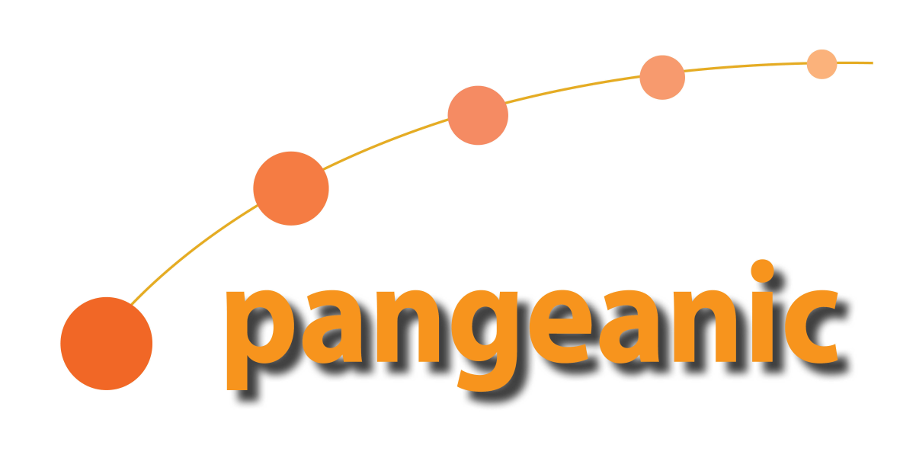
\includegraphics[width=0.8\columnwidth]{logos/pangeanic-logo.png}

\vfill

\includegraphics[width=0.8\columnwidth]{logos/yamagata-logo.png}
\end{center}

\vfill

\newpage

\section*{Bronze sponsors}
\vfill

\begin{center}

\includegraphics[width=0.60\columnwidth]{logos/star-logo.jpg}

\vfill


\includegraphics[width=0.75\columnwidth]{logos/unbabel-logo.png}

\vfill

\includegraphics[width=0.65\columnwidth]{logos/welocalize-logo.png}

\end{center}
\vfill
\newpage

\section*{Collaborator sponsors}
\begin{center}

\includegraphics[width=0.55\columnwidth]{logos/apertium-logo.png}
\end{center}

\vfill

\section*{Supporter sponsors}
\begin{center}
\includegraphics[width=0.50\columnwidth]{logos/springer-logo.png}
\end{center}

\vfill

\section*{Media sponsors}
\begin{center}

\includegraphics[width=0.50\columnwidth]{logos/multilingual-logo.png}
\end{center}

\newpage
\section*{Institutional partners}

\begin{center}
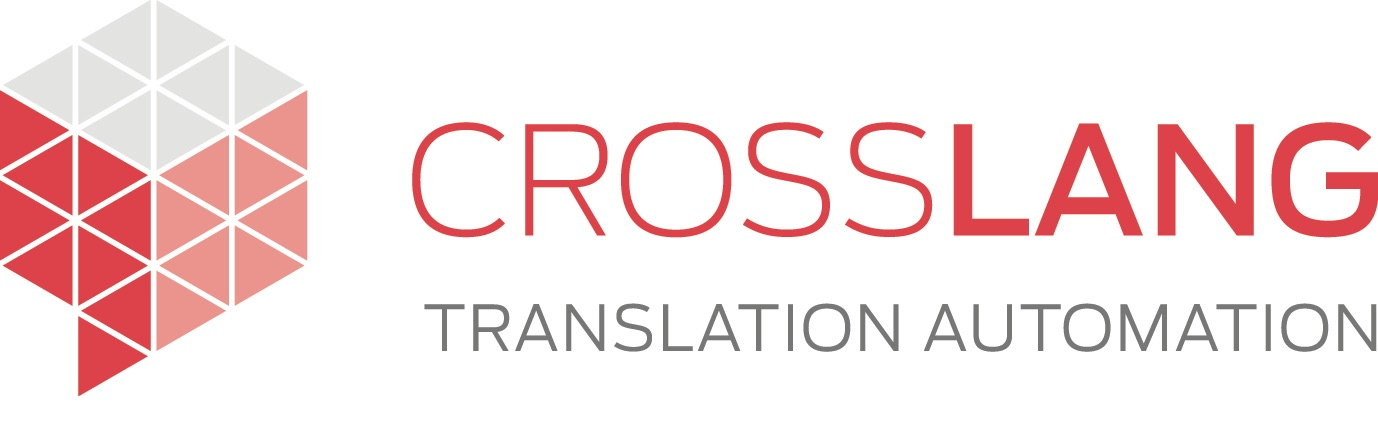
\includegraphics[width=0.5\columnwidth]{logos/crosslang-logo.png}\\
\vfill

\includegraphics[width=0.4\columnwidth]{logos/lt3-text-logo.png}\\
\vfill

\includegraphics[width=0.3\columnwidth]{logos/ugent-logo.png}
\end{center}

\vfill

\end{document}